\chapter{Επίδειξη της εφαρμογής(\en{Application Demo})}

\section{Εισαγωγή-Η λογική της λειτουργίας της εφαρμογής \en{Django}}

Όταν τρέχουμε τον διακομιστή της εφαρμογής η εφαρμογή ιστού
είναι διαθέσιμη από οποιοδήποτε φυλλομετρητή. Η αρχική σελίδα στη εφαρμογή
\en{Django} δηλώνεται στο πλαίσιο του \en{Django run server} ώς μία συνάρτηση της \en{Python}
η οποία δέχεται ένα \en{http request} και σαν απάντηση επιστρέφει την αρχική σελίδα(\en{index.html}).

Αυτό γίνεται μέσα από 2 κύριως μηχανισμούς.Η συνάρτηση \en{firstPage} ορίζεται στο αρχείο \en{views.py} της εφαρμογής. Παίρνει ως όρισμα ένα αντικείμενο \en{HttpRequest} 
(την αίτηση του χρήστη) και επιστρέφει ένα \en{HttpResponse} μέσω της \en{render}(σχήμα 7.1):

\FloatBarrier
\begin{figure}[h]
	\centering
	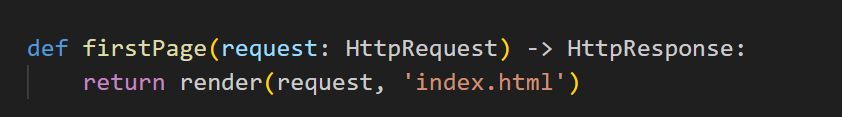
\includegraphics[width=1.0\textwidth]{graphics/firstPage.png}
	\caption{ \en{firstPage} συνάρτηση}
\end{figure}

\FloatBarrier

Η λίστα \en{urlpatterns} συνδέει τη διεύθυνση \en{URL} 
με τη συνάρτηση \en{firstPage}. Το κενό \en{string} ('') σημαίνει ότι αυτή η διαδρομή αντιστοιχεί στη ρίζα του ιστότοπου (π.χ., \en{http://localhost:8000/})
Όταν ένας χρήστης επισκέπτεται τη ρίζα, η συνάρτηση \en{firstPage} 
εκτελείται και επιστρέφει την \en{HTML} σελίδα \en{index.html}. Στο σχήμα 7.2 το σημείο στο \en{urls.py} όπου γίνεται η δρομολόγηση.

\FloatBarrier

\begin{figure}[h]
	\centering
	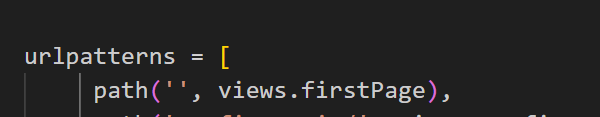
\includegraphics[width=1.0\textwidth]{graphics/urls_firstPage.png}
	\caption{ \en{Urls} δρομολόγηση για την αρχική σελίδα.}
\end{figure}

\FloatBarrier

Μέσα από αυτή την αρχική σελίδα μπορούμε να κατευθυνθούμε σε οποιαδήποτε επιλογή εμείς θέλουμε.
Στο \en{Django} καθοριστικός παράγοντας στην ευκολία με την οποία
μπορείς να χτίσεις μια εφαρμογή από την αρχή είναι ο τρόπος που χειρίζεται
τη δρομολόγηση των διαφόρων σελίδων. Αυτό γίνεται μεσα απο το \en{urls.py}

Αυτή η ρύθμιση καθορίζει πώς θα δρομολογούνται οι 
αιτήσεις \en{HTTP} προς συγκεκριμένες λειτουργίες (\en{views}) 
στην εφαρμογή \en{Django}. Με τη χρήση των δυναμικών παραμέτρων, 
μπορούμε συνεπώς να δημιουργήσουμε πιο ευέλικτες διαδρομές \en{URL} 
που μπορούν να χειρίζονται ποικίλες καταστάσεις. 

Κάθε ένα από αυτά τα \en{paths} που φαίνονται και στην εικόνα 7.3
είναι υπεύθυνα για την ανακατεύθυνση των διευθύνσεων και τη σωστή δρομολόγησή
τους ώστε να δώσουν σαν απάντηση κάθε φορά τα σωστά δεδομένα.

\FloatBarrier
\begin{figure}[h]
	\centering
	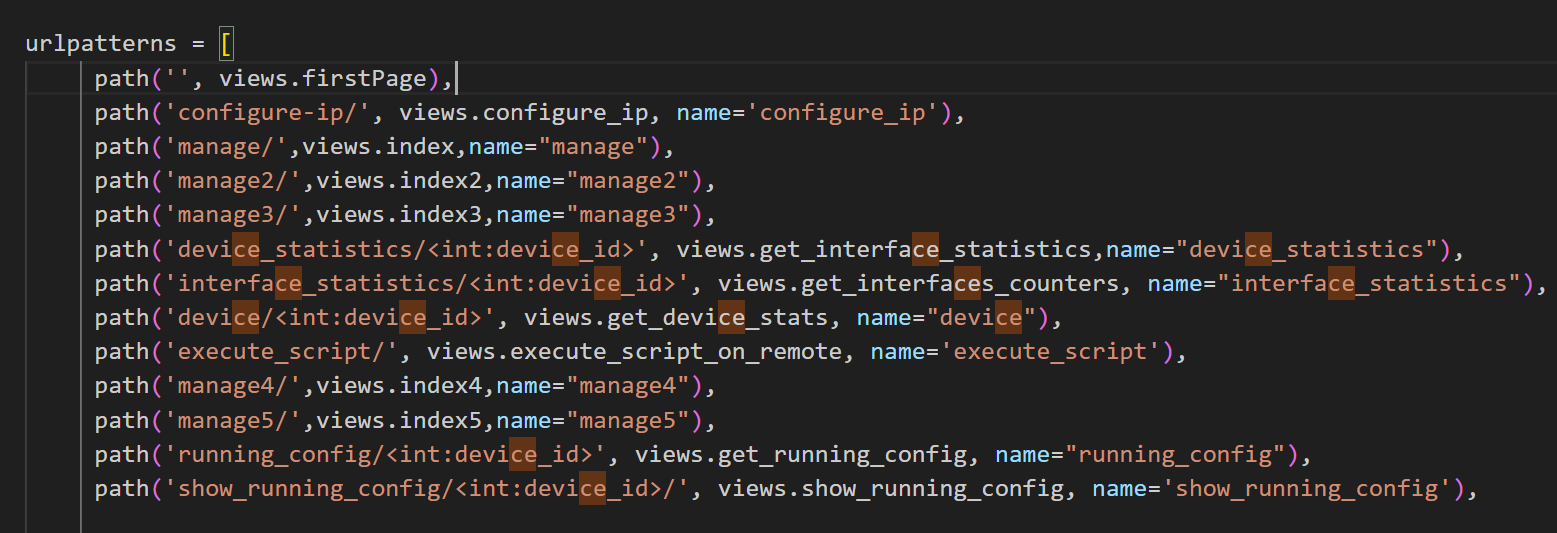
\includegraphics[width=1.0\textwidth]{graphics/urls.png}
	\caption{ \en{Urls.py} αρχείο}
\end{figure}

\FloatBarrier



\section{Η αρχική σελίδα της εφαρμοφής}

Προκειμένου να τρέξει ο \en{Django server}
τρέχουμε την εντολή η οποία βρίσκεται στην 
εικόνα 7.4.

\begin{figure}[h]
	\centering
	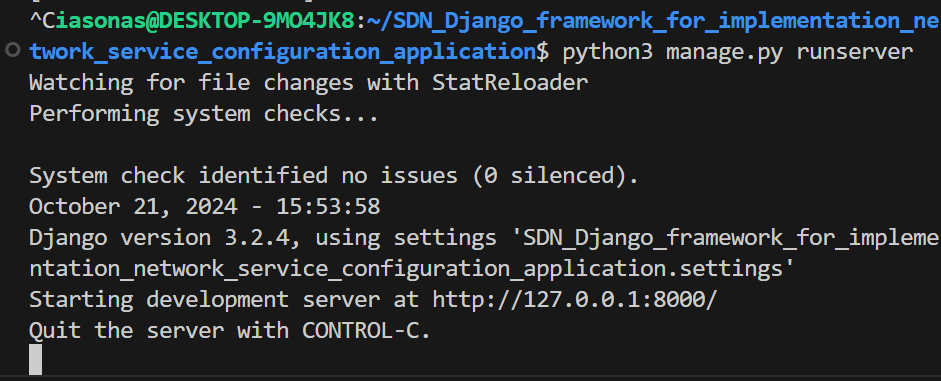
\includegraphics[width=1.0\textwidth]{graphics/django_server_run.png}
	\caption{ \en{Django run server}}
\end{figure}






Ο εξυπηρετητής τρέχει σαν διεργασία στο λειτουργικό
και είναι διαθέσιμος στη διεύθυνση \en{http://127.0.0.1:8000/}

Εάν εισάγουμε αυτή τη διεύθυνση σε έναν 
φυλλομετρητή της επιλογής μας, θα ανακατευθυνθούμε 
στην αρχική σελίδα, η οποία θα παρουσιαστεί στον 
χρήστη όπως στην εικόνα 7.5. Το εμπρόστιο τμήμα της εφαρμοφής(\en{frontend}) 
είναι γραμμένο με \en{HTML},\en{CSS} ενώ το οπίσθιο τμήμα(\en{backend}) 
είναι γραμμένο σε \en{Python}.

\FloatBarrier
\begin{figure}[h]
	\centering
	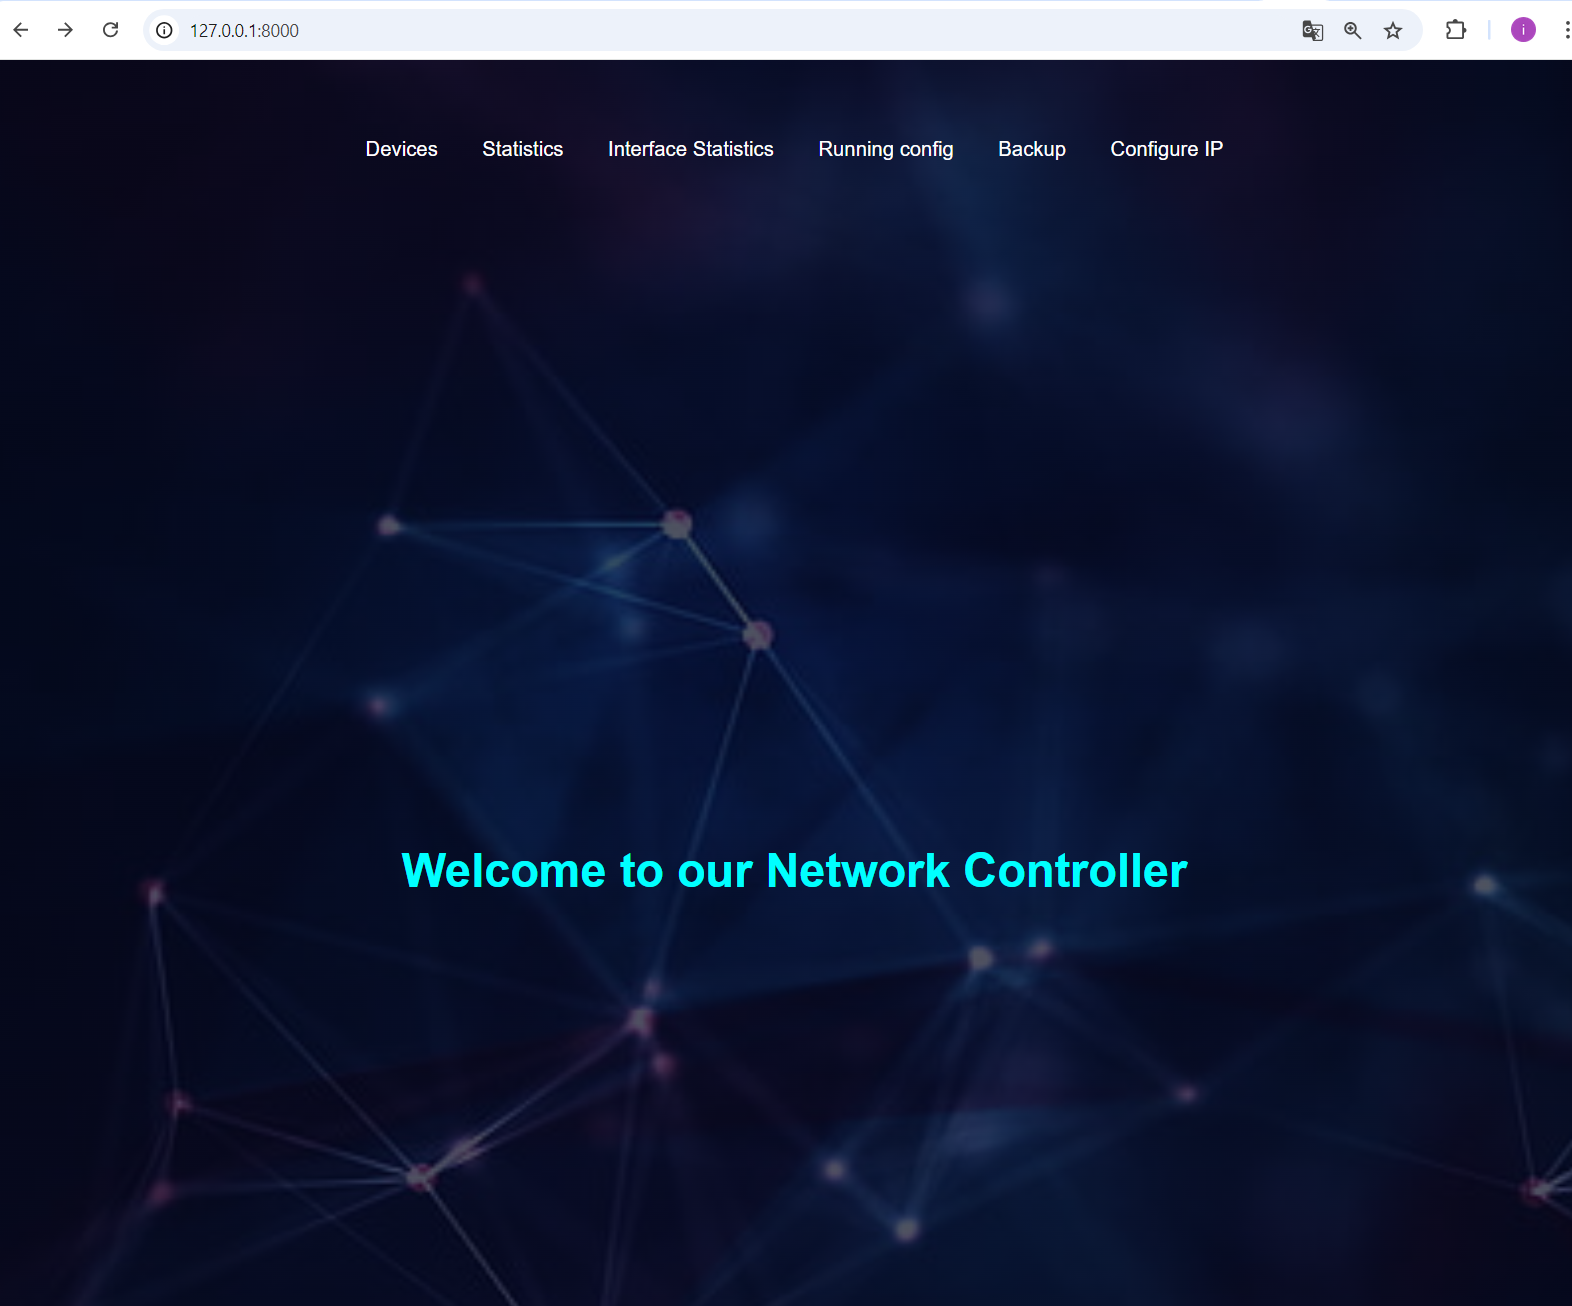
\includegraphics[width=1.2\textwidth]{graphics/home_page.png}
	\caption{ Αρχική Σελίδα}
\end{figure}

\FloatBarrier % Prevents floats from moving past this point

\section{\en{Devices}}

Προκειμένου να δημιουργήσουμε μία νεα συσκευή η παρακατω κλάσση
κώδικα μας βοηθάει στο να γίνει όπως στο σχήμα 7.6.

\FloatBarrier
\begin{figure}[htb]
	\centering
	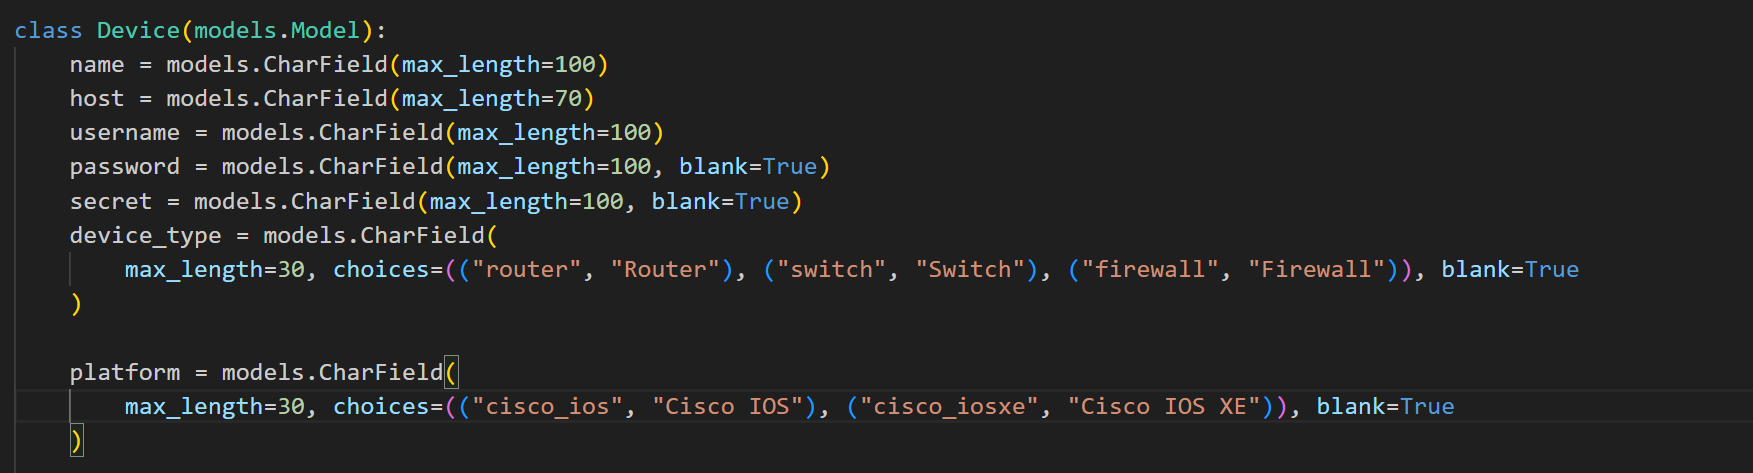
\includegraphics[width=1.2\textwidth]{graphics/class_device.png}
	\caption{Αρχικοποίηση συσκευής}
\end{figure}

\FloatBarrier

Αφού λοιπόν πατήσουμε το κουμπί \en{Devices} αυτό θα μας δρομολογήσει στο αντίστοιχο \en{HTML link}.
Το οποίο θα μας εμφανίσει μια άλλη σελίδα αυτή του σχήματος 7.7. 

Αποτέλεσμα του πίνακα του σχήματος 7.7 είναι όλες οι συσκευές οι οποίες
είναι στη βάση δεδομένων μας όπου ο χρήστης πρόσθεσε προκειμένου
να μπορεί να αναδράσει με αυτές. Το πως προσθέτουμε συσκευές αναλύθηκε στ προηγούμενο κεφάλαιο αναλυτικά.

\FloatBarrier
\begin{figure}[htb]
	\centering
	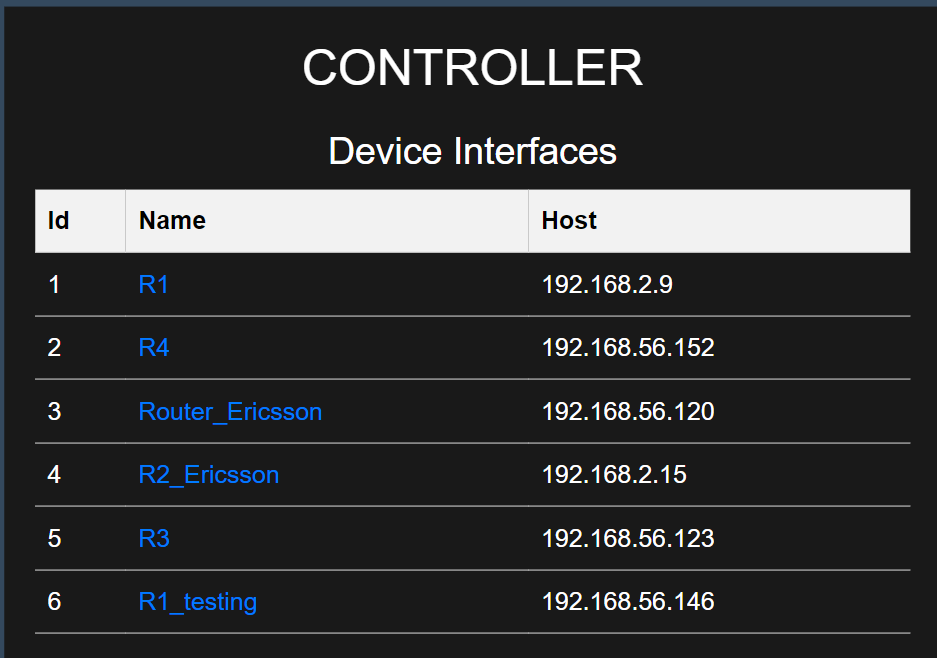
\includegraphics[width=1.2\textwidth]{graphics/device_interfaces.png}
	\caption{\en{Controller-Device Interfaces}}
\end{figure}

\FloatBarrier

Πατόντας ένα από αυτά τα κουμπιά θα μπορέσουμε να πάρουμε το αποτέλεσμα που θέλουμε.
Σε αυτή τη σελίδα μπορούμε να δούμε αν κάποια διεπαφή αν λειτουργεί ή όχι.
(Σχήμα 7.8)

\FloatBarrier
\begin{figure}[htb]
	\centering
	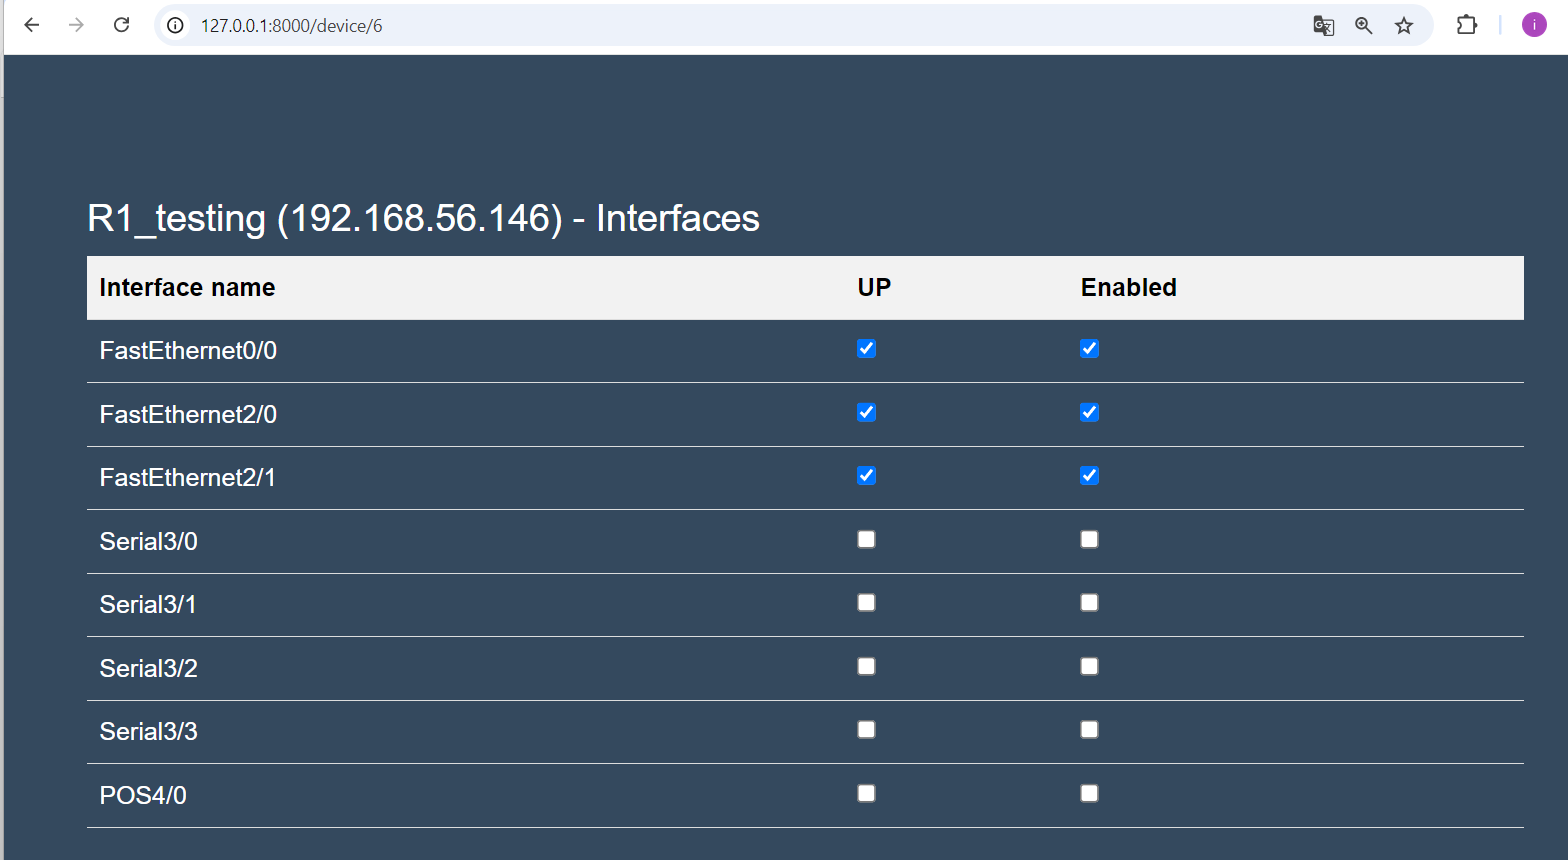
\includegraphics[width=1.2\textwidth]{graphics/interfaces.png}
	\caption{\en{Interfaces}}
\end{figure}
\FloatBarrier


\section{Στατιστικά της συσκευής}

Η λειτουργία του κουμπιού \en{Statistics} βασίζεται στη συνάρτηση \en{get\_interface\_statistics}, 
η οποία είναι υπεύθυνη για τη σύνδεση σε μια δικτυακή συσκευή, 
την απόκτηση στατιστικών πληροφοριών σχετικά με τις 
διεπαφές της, και την παρουσίαση αυτών των πληροφοριών 
σε μια ιστοσελίδα μέσω ενός προτύπου \en{HTML}. Η συνάρτηση αυτή 
δέχεται δύο παραμέτρους: το αίτημα του χρήστη (\en{request}) 
και το αναγνωριστικό της συσκευής (\en{device\_id}), 
το οποίο χρησιμοποιείται για να εντοπίσει τη συγκεκριμένη 
συσκευή από τη βάση δεδομένων.

Για να εντοπίσει τη συσκευή, παρουσιάζεται μία λίστα από το 
\en{User Interface} όπως και στην εικόνα (\en{Devices}) 7.9.


\FloatBarrier

\begin{figure}[h]
	\centering
	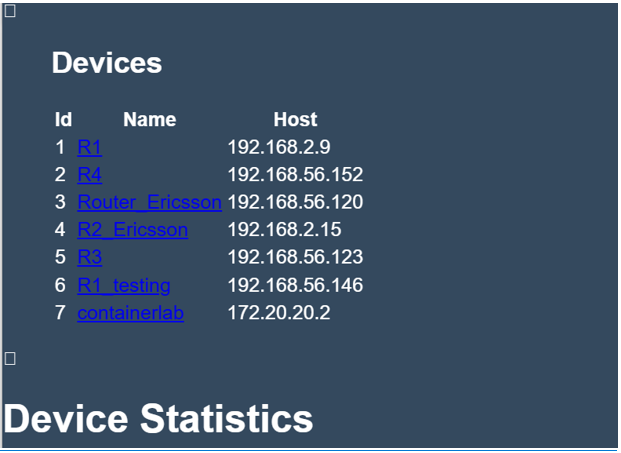
\includegraphics[width=1.0\textwidth]{graphics/device_statistics.png}
	\caption{Στατιστικά Συσκευής}
\end{figure}

\FloatBarrier

Πατώντας πάνω σε κάθε μια από τις συσκευές που έχουμε ορίσει και εμφανίζονται ως \en{links} εµφανίζει τα παρακάτω στατιστικά αντίστοιχα. Όπως στην  εικόνα 7.10.


\FloatBarrier

\begin{figure}[h]
	\centering
	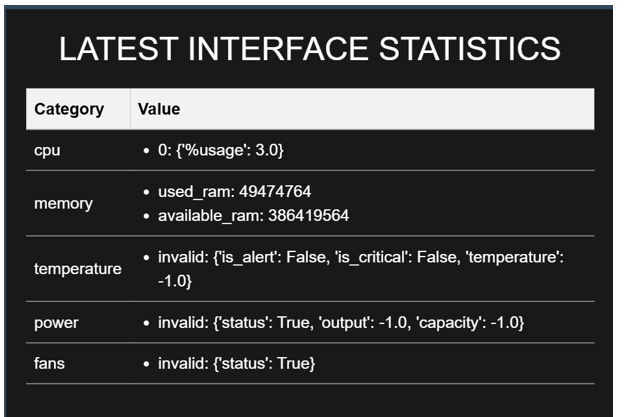
\includegraphics[width=1.0\textwidth]{graphics/device_statistics_response.png}
	\caption{Στατιστικά Συσκευής}
\end{figure}

\FloatBarrier


\section{Στατιστικά της διεπαφής}

Η συνάρτηση επιτρέπει τη σύνδεση σε μια δικτυακή συσκευή, την ανάκτηση των στατιστικών των διεπαφών της και την παρουσίαση αυτών των δεδομένων σε μια ιστοσελίδα

\FloatBarrier

\begin{figure}[h]
	\centering
	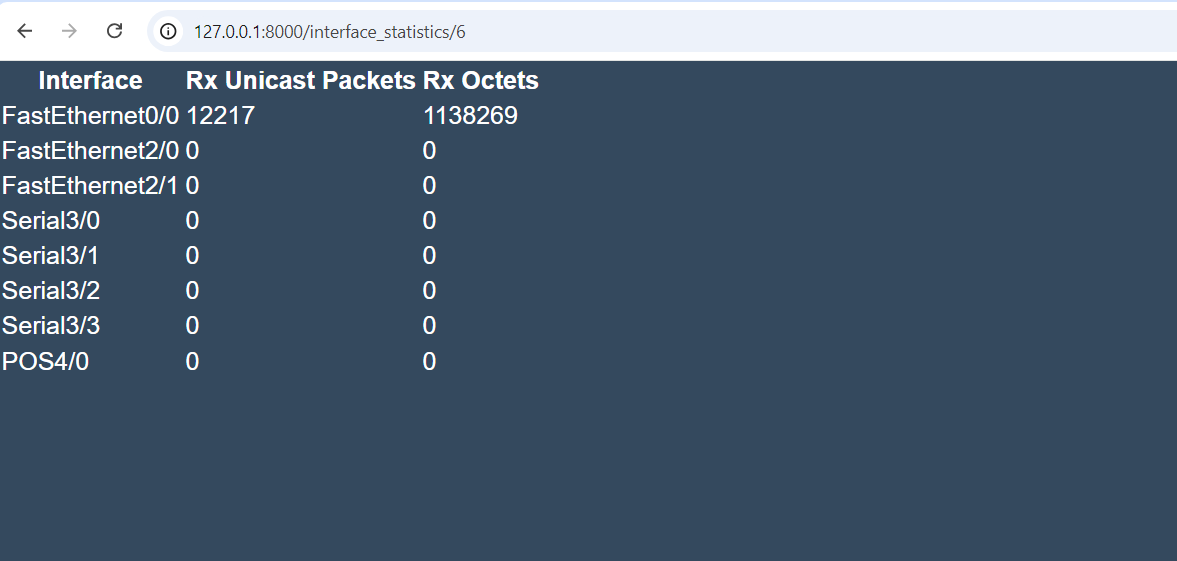
\includegraphics[width=1.0\textwidth]{graphics/interface_statistics.png}
	\caption{Στατιστικά διεπαφής}
\end{figure}


\section{\en{Backup} της συσκευής}

Προκειμένου να σώσουμε τη διαμόρφωση της συσκευής πατάμε το κουμπί
\en{backup} και με αυτό πέρνουμε το παρακάτω αποτέλεσμα.

Ουσιαστικά είναι σε \en{text} αρχείο το λεγόμενο \en{running config}
της συσκευής

\FloatBarrier

\begin{figure}[h]
	\centering
	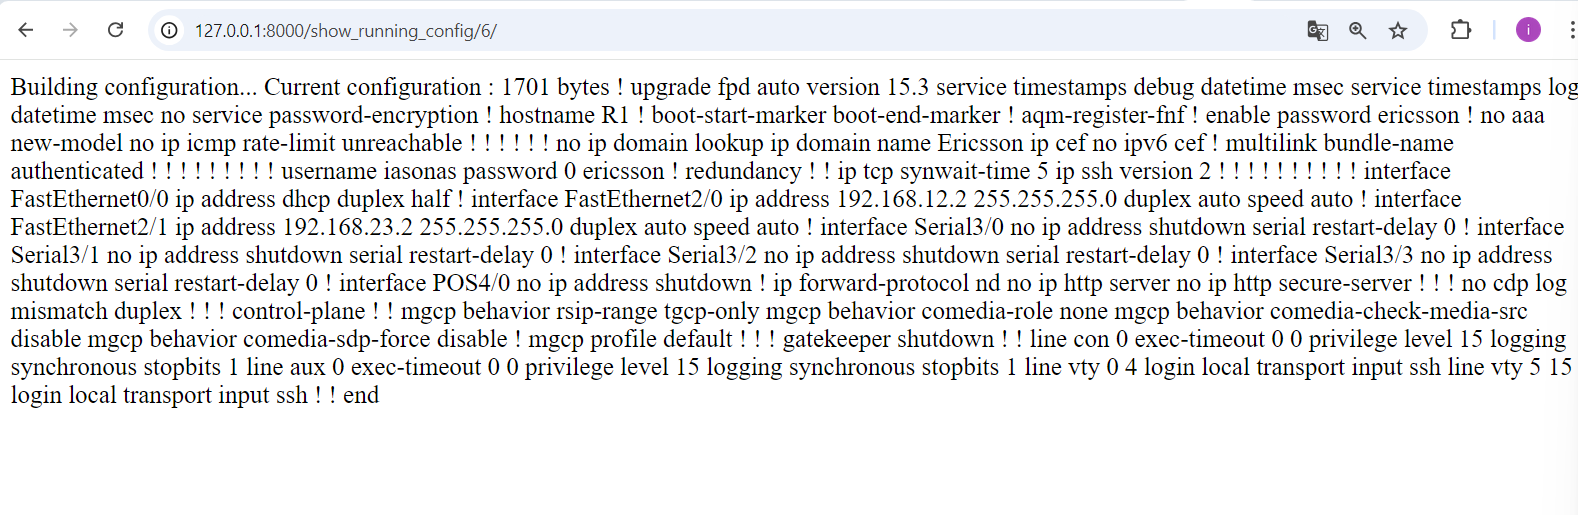
\includegraphics[width=1.0\textwidth]{graphics/running_config.png}
	\caption{Τρέχων Διαμόρφωση}
\end{figure}


\section{Διαμόρφωση διεύθυνσης \en{IP}}

Η διαμόρφωση \en{IP} διεύθυσης γίνεται δίνοντας τα παρακάτω στοιχεία
σαν είσοδο

\FloatBarrier

\begin{figure}[h]
	\centering
	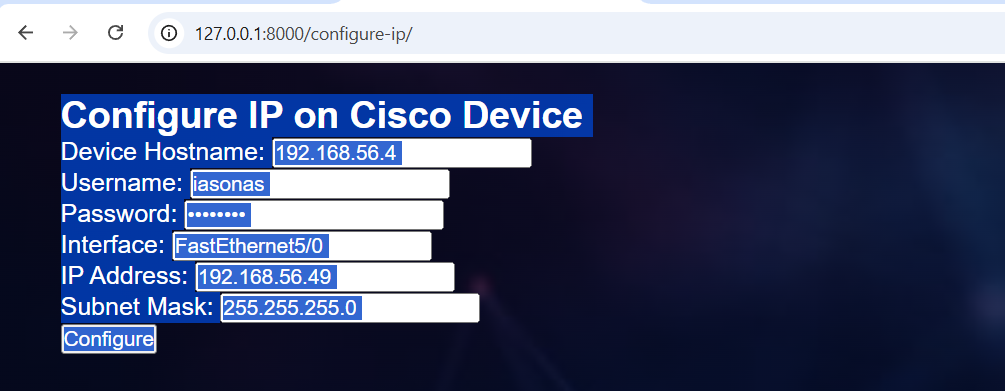
\includegraphics[width=1.0\textwidth]{graphics/configure_ip.png}
	\caption{\en{IP}Διαμόρφωση}
\end{figure}

Και καταφέρνει και αλλάζει την διέυθυνση.

\FloatBarrier

\begin{figure}[h]
	\centering
	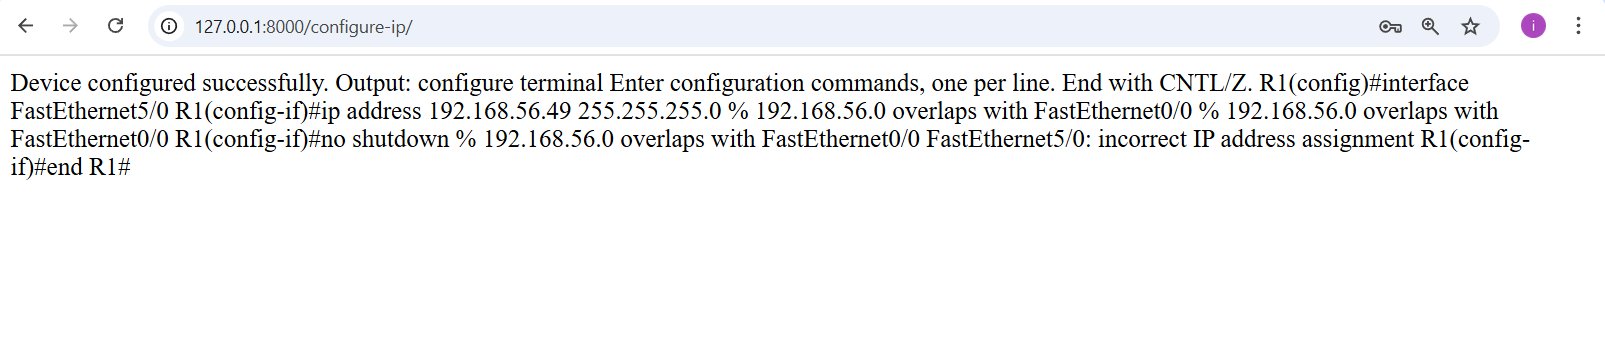
\includegraphics[width=1.0\textwidth]{graphics/configure_ip_1.png}
	\caption{\en{IP} Διαφορά}
\end{figure}